% !TEX TS-program = xelatex
% !TEX encoding = UTF-8
% !Mode:: "TeX:UTF-8"

\documentclass[onecolumn,oneside]{BUPTHomework}

\usepackage{blindtext}

\author{胡玉斌}
\sid{2021111054}
\title{Review\ 第七章\ Turbo码}
\coursecode{3131100063}
\coursename{编码理论}

\begin{document}
  \maketitle
  
  \section*{Turbo码背景介绍}

  根据 Shannon 有噪信道编码定理,
  在信道传输速率 R 不超过信道容量 C 的前提下,
  只有在码组长度无限的码集合中随机地选择编码码字并且在接收端采用最大似然译码算法时,
  才能使误码率接近为零。

  Turbo 码,由于它很好地应用了 shannon 信道编码定理中的随机性编、译码条件,从而获得了几乎接近 shannon 理论极限的译码性能

  Turbo 码又称并行级联卷积码 (PCCC,Parallel Concatenated Convolutional Code),
  它巧妙地将卷积码和随机交织器结合在一起,
  在实现随机编码思想的同时,
  通过交织器实现了由短码构造长码的方法,
  并采用软输出迭代译码来逼近最大似然译码。

  \section*{Turbo码的编码}

  Turbo 码的编码结构可以分为并行级联卷积码(PCCC)、串行级联卷积码(SCCC)和混合级联卷积码(HCCC)三种。

  我们主要讨论 PCCC 结构的卷积码。

  $$u=(u_0,u_1,⋯,𝑢_{𝐾−1})$$

  \begin{enumerate}
    \item 为了得到靠近Shannon限的系统性能,信息分组长度K一般比较大,通常至少几千个比特。
    \item 对于分量码来说,一般选择相同结构,且约束长度较短,通常v≤4。 
    \item 递归分量码(由系统反馈编码器产生)会比非递归分量码(前馈编码器)有更好的性能;
    \item 高码率可通过穿刺矩阵产生
    \item 通过增加分量码和交织器也可得到较低编码速率的 Turbo 码
    \item 最好的交织器能够对比特以伪随机的方式进行排序,传统的块交织器(行-列)在 Turbo 码中性能不好,除非 block 长度很短;
    \item 由于交织器只是对比特位置进行重新排序,因此,交织后的序列u′与原始序列 u 具有相同的重量;
    \item 对每个分量码来说,用 BCJR(或 MAP)算法作为 SISO 译码器能够获得最好的性能;因为 MAP 译码器使用了前向-后向算法,信息是以 block 的形式进行的,因此,对第一个分量译码器来说,附加 v 个 0 比特能够让它返回到全 0 态;但对于第二个译码器来说,由于交织器的作用,将不能返回到全 0 态。
  \end{enumerate}

  \subsection*{缺点}

  \begin{itemize}
    \item 较大的译码时延,这是由于 block 长度较大、译码需要多次迭代造成的。
    \item BER 在 10-5 后会出现误码平台,这是由于 Turbo码的重量分布造成的。对于某些对 BER 要求较高的应用就不适合。
  \end{itemize}

  \section*{Turbo码的译码}

  \begin{figure}[!htbp]
    \centering
    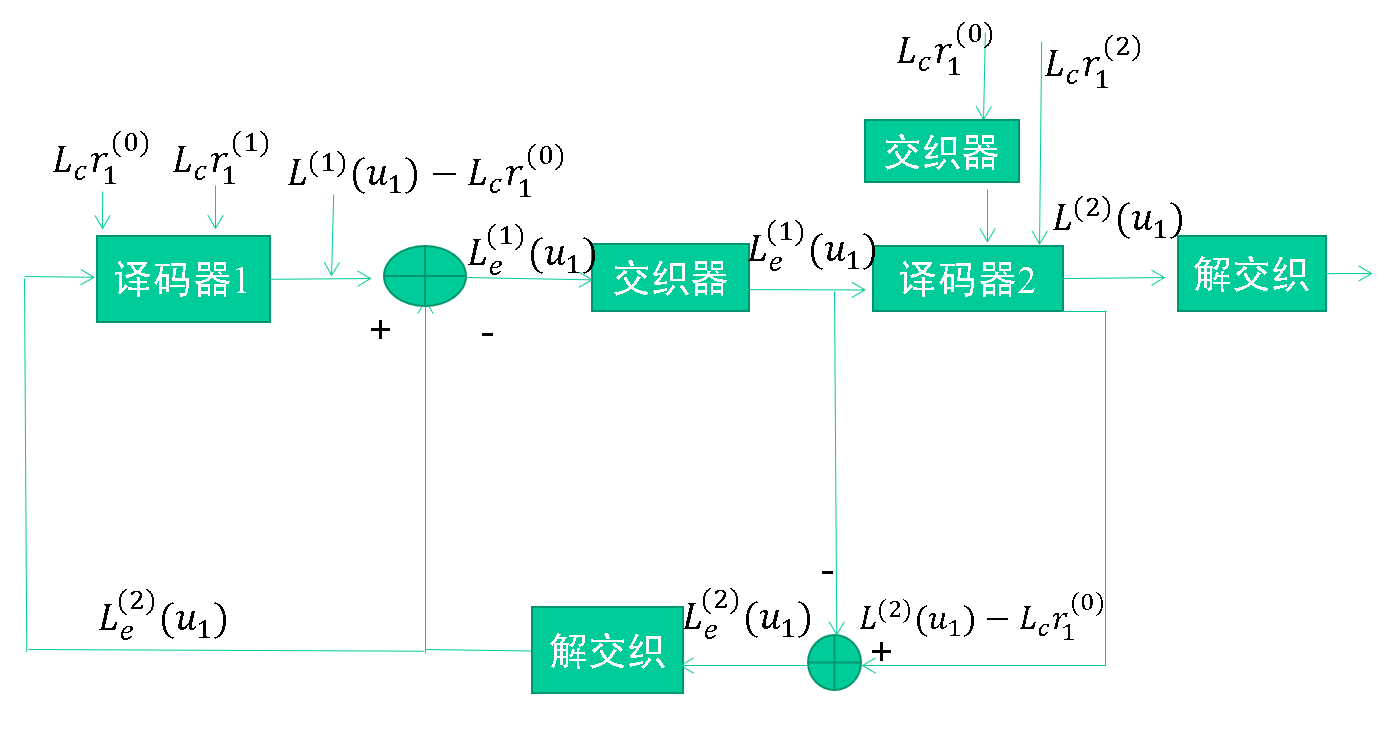
\includegraphics[width = 12cm ]{image/pic1.png}
    \caption{迭代译码器的基本结构}
  \end{figure}

  \section*{心得体会\&建议}

  \begin{enumerate}
    \item 讲课效果一般
  \end{enumerate}
  
\end{document}
